\documentclass[12pt,article]{article}
\usepackage{lmodern}
\usepackage{amssymb,amsmath}
\usepackage{ifxetex,ifluatex}
\usepackage{fixltx2e} % provides \textsubscript
\ifnum 0\ifxetex 1\fi\ifluatex 1\fi=0 % if pdftex
  \usepackage[T1]{fontenc}
  \usepackage[utf8]{inputenc}
\else % if luatex or xelatex
  \ifxetex
    \usepackage{mathspec}
    \usepackage{xltxtra,xunicode}
  \else
    \usepackage{fontspec}
  \fi
  \defaultfontfeatures{Mapping=tex-text,Scale=MatchLowercase}
  \newcommand{\euro}{€}
\fi
% use upquote if available, for straight quotes in verbatim environments
\IfFileExists{upquote.sty}{\usepackage{upquote}}{}
% use microtype if available
\IfFileExists{microtype.sty}{%
\usepackage{microtype}
\UseMicrotypeSet[protrusion]{basicmath} % disable protrusion for tt fonts
}{}
\usepackage[margin=1in]{geometry}
\ifxetex
  \usepackage[setpagesize=false, % page size defined by xetex
              unicode=false, % unicode breaks when used with xetex
              xetex]{hyperref}
\else
  \usepackage[unicode=true]{hyperref}
\fi
\hypersetup{breaklinks=true,
            bookmarks=true,
            pdfauthor={Justin Murphy; Daniel Devine},
            pdftitle={Does Public Support for UKIP Drive Their Media Coverage or Does Media Coverage Drive Support for UKIP?},
            colorlinks=true,
            citecolor=blue,
            urlcolor=blue,
            linkcolor=blue,
            pdfborder={0 0 0}}
\urlstyle{same}  % don't use monospace font for urls
\usepackage{graphicx,grffile}
\makeatletter
\def\maxwidth{\ifdim\Gin@nat@width>\linewidth\linewidth\else\Gin@nat@width\fi}
\def\maxheight{\ifdim\Gin@nat@height>\textheight\textheight\else\Gin@nat@height\fi}
\makeatother
% Scale images if necessary, so that they will not overflow the page
% margins by default, and it is still possible to overwrite the defaults
% using explicit options in \includegraphics[width, height, ...]{}
\setkeys{Gin}{width=\maxwidth,height=\maxheight,keepaspectratio}
\setlength{\parindent}{0pt}
\setlength{\parskip}{6pt plus 2pt minus 1pt}
\setlength{\emergencystretch}{3em}  % prevent overfull lines
\providecommand{\tightlist}{%
  \setlength{\itemsep}{0pt}\setlength{\parskip}{0pt}}
\setcounter{secnumdepth}{0}

%%% Use protect on footnotes to avoid problems with footnotes in titles
\let\rmarkdownfootnote\footnote%
\def\footnote{\protect\rmarkdownfootnote}

%%% Change title format to be more compact
\usepackage{titling}

% Create subtitle command for use in maketitle
\newcommand{\subtitle}[1]{
  \posttitle{
    \begin{center}\large#1\end{center}
    }
}

\setlength{\droptitle}{-2em}
  \title{Does Public Support for UKIP Drive Their Media Coverage or Does Media
Coverage Drive Support for UKIP?}
  \pretitle{\vspace{\droptitle}\centering\huge}
  \posttitle{\par}
  \author{Justin Murphy \\ Daniel Devine}
  \preauthor{\centering\large\emph}
  \postauthor{\par}
  \date{}
  \predate{}\postdate{}

\usepackage{dcolumn}
\usepackage{setspace}
\usepackage{hyperref}

% Redefines (sub)paragraphs to behave more like sections
\ifx\paragraph\undefined\else
\let\oldparagraph\paragraph
\renewcommand{\paragraph}[1]{\oldparagraph{#1}\mbox{}}
\fi
\ifx\subparagraph\undefined\else
\let\oldsubparagraph\subparagraph
\renewcommand{\subparagraph}[1]{\oldsubparagraph{#1}\mbox{}}
\fi

\begin{document}
\maketitle

\begin{abstract}
Previous research suggests media attention may cause support for populist right-wing parties, but extant evidence remains arguable and mostly limited to proportional representation systems in which such an effect would be most likely. At the same time, in the United Kingdom's first-past-the-post system, an ongoing political and regulatory debate revolves around whether the media give disproportionate coverage to the populist right-wing UK Independence Party (UKIP). Thus, we use a mixed-methods approach to investigate the causal dynamics of UKIP support and media coverage as an especially valuable case. Vector autoregression (VAR) using monthly, aggregate time-series data from January 2004 to September 2015 provides new evidence consistent with a model in which media coverage drives party support, but party support does not drive media coverage. Additionally, qualitative investigation of the dynamics suggests that in at least two key periods of stagnating or declining support for UKIP, media coverage increased and was followed by increases in public support. Overall the findings show that media coverage can and does appear to drive public support in a substantively important fashion irreducible to previous levels of public support, even in a national institutional environment least supportive of such an effect. The findings have direct and troubling implications for contemporary political and regulatory debates in the United Kingdom and potentially liberal democracies more generally.\footnote{Justin Murphy (\href{http://jmrphy.net}{jmrphy.net}, \href{http://twitter.com/jmrphy}{@jmrphy}) is Assistant Professor of Politics at the University of Southampton. Daniel Devine is a post-graduate researcher at the University of Southampton. This manuscript was prepared for the 2016 annual meeting of the Political Studies Association in Brighton, UK. Comments, questions, and suggestions are welcome and can be emailed to \href{mailto:j.murphy@soton.ac.uk}{j.murphy@soton.ac.uk}. If you wish to cite, please use the citation and DOI provided with the most up-to-date version of this article, which will be maintained at \href{http://j.mp/ukip-media}{j.mp/ukip-media}.}
\end{abstract}
\doublespacing
\setlength\parindent{24pt}

\section{Introduction}\label{introduction}

If the visibility of a political party in the media shapes the public
support it receives, then the degree to which the media gives attention
to different political parties can have significant implications for
democracy. In the United Kingdom, critics allege that the media pays
disproportionate attention to the populist, right-wing UK Independence
Party (UKIP) but media elites claim that media coverage of UKIP is
driven by increasing public support for the party. Descriptively, media
attention to UKIP is greater than that given to other, similarly sized
parties on the right as well as the left (Goodwin and Ford, 2013;
Stevenson, 2014; Soussi, 2014), but UK media regulator Ofcom as well as
the BBC have publicly defended the attention paid to UKIP on grounds of
public support for the party (Sweeney, 2015; Wintour, 2015). Implied in
this elite reasoning is a causal model, namely that public support
drives media coverage rather than vice-versa.

Yet previous research from proportional representation systems suggests
that public support does not drive media coverage for populist
right-wing parties, but rather media coverage drives their public
support (Boomgaarden and Vliegenthart, 2007, 2009; Vliegenthart et al.,
2012). By leveraging this insight to investigate the causal dynamics of
UKIP support and media coverage, we fill an important gap in current
research on the visibility-support nexus and contribute pragmatically
relevant insights to a contentious public policy debate of broad social
significance (Gerring, 2015). First, we contribute to current research
on the visibility-support nexus by testing a key insight from this
research in a new institutional context where the hypothesized
relationship should be less likely. Because proportional representation
systems are associated with a greater number of small parties (Duverger,
1972) and they tend to produce more diverse news (Benson, 2009; Sheafer
and Wolfsfeld, 2009; Kumlin, 2001; Strömbäck and Dimitrova, 2006; Baum,
2012), research confined to such systems is arguably most likely to
reflect a model in which media coverage generates support for populist
right-wing parties. In a first-past-the-post system, where we typically
expect only two parties and media to be less diverse, these
institutional pressures make it more difficult for the media to generate
support for smaller populist, right-wing parties. Thus, testing this
theory with time-series data from a first-past-the-post system
contributes to either refining the scope conditions of previous research
(in the case of unexpected findings) or else extending and strengthening
our confidence in the media-support relationship. Secondly, we
contribute to a pressing regulatory question in UK national politics, as
the democratic quality of UK media regulation with respect to political
party favouritism, especially regarding populist right-wing parties,
remains on public trial. This article lends insight into the causal
dynamics implied but rarely if ever tested within such popular policy
debates.

The article begins by outlining the theory before moving to a discussion
of our data, method and research strategy. We then present quantitative
and qualitative analyses of the relationship between UKIP support and
UKIP media coverage. A final section concludes.

\section{Theory}\label{theory}

A large body of research suggests that mass media coverage, as the
primary channel through which the electorate receives information about
politicians and parties, affects many different aspects of electoral
politics (Norris, 2000; Paletz, 1996; Beck et al., 2002; Dalton et al.,
1998). If media coverage of political parties is driven by public
support for the parties--even if media coverage then increases public
support further--it could be argued that media are facilitating popular
sovereignty. On the other hand, if media coverage independently changes
public support rather than reflects it, this would represent a point of
crucial possible distortion in the functioning of a democracy. The
latent normative motivation for the present investigation is whether the
quantity of UKIP's media coverage represents a form of media bias which
generates rather than reflects public opinion, or if the media's
fascination with UKIP is a democratically appropriate effect of public
opinion.

One current of previous research on the dynamics of media coverage and
party support finds evidence consistent with the argument that the
quantity of media coverage given to a political party drives public
support for that party. Walgrave and De Swert (2004) find that, in
time-series data from Belgium, the evidence reflects a model in which
newspapers and television stations helped to increase the electoral
results of the Vlaams Blok by emphasising political issues owned by the
extreme right-wing party. Boomgaarden and Vliegenthart (2007;
Vliegenthart and Boomgaarden, 2010) find that in the Netherlands,
quantity of media coverage on immigration-related topics is associated
with a subsequent increase in the vote-share for anti-immigrant parties,
controlling for objective factors such as levels of immigration.
Boomgaarden and Vliegenthart (2009) also find, using time-series from
Germany, that media coverage of immigrant actors is associated with
subsequent change in public attitudes toward immigration, conditional on
objective factors such as immigration levels. While much of the previous
research above considers the political implications of issue coverage in
the media, Vliegenhart, Boomgaarden, and Van Spanje (2012) advance this
current further by analyzing time-series on the coverage of parties and
public support for anti-immigrant parties per se in Belgium,
Netherlands, and Germany. That study finds evidence suggesting that
party and party leader visibility is associated with the electoral
outcomes of the parties, but not vice-versa. In another study, media
coverage was found to be one of the best predictors of electoral success
in the 2007 Dutch election (Hopmann et al., 2010). Finally, it has been
shown that in the Netherlands, media coverage of Fortuyn appears to have
improved polling performance of the party before the 2002 election
(Koopmans and Muis, 2009).

Considering research at the individual level, panel data from the
Netherlands suggests that media coverage drives perceptions of
right-wing populist politicians as well as mainstream politicians (Bos
et al., 2011). Media coverage has also been found to help explain
individual-level party preferences in Germany (Semetko and Schoenbach,
1994) and the Netherlands (Oegema and Kleinnijenhuis, 2009). Based on
this previous research, we test the following hypothesis.

H1: \emph{Increases in media coverage lead to increased public support,
controlling for previous levels of public support.}

It is also theoretically plausible, as some scholars have argued, that
changes in party support lead to changes in media coverage (Pauwels,
2010). As Vliegenthart and Boomgaarden (2010) consider, quantity of
media coverage may be driven by the power and position of political
figures. This pattern has been observed, in some cases, in America
(Sellers and Schaffner, 2007) and Switzerland (Tresch, 2009). Sellers
(2007) finds that the types of events U.S. Senators hold, and the guests
of those events, affects the number of news stories written. Tresch
(2009) finds that the amount of coverage given to Swiss legislators is
most importantly a function of leadership and authority criteria related
to the individual politicians. Although both of these studies focus on
politicians rather than political parties per se, they suggest that
variable aspects of political entities have predictable effects on media
visibility. In a study on the diffusion of populist discourse in the
media, Rooduijn (2014) argues from a study of five Western European
countries (Italy, France, Germany, Netherlands, and United Kingdom) the
electoral success of populist parties affects the degree of populism in
the
media.\footnote{Interestingly, in the study by Rooduijn, UKIP is classified as the least successful case of a populist party, based on their electoral results as of 2005, yet populism in British newspapers in 2005 is near that found in Netherlands and Germany and greater than that found in France. Although the findings are interpreted as electoral politics driving media content, Rooduijn's data show that in the UK at least, populism in the media was comparatively high in cross-national perspective before UKIP rose to its recent prominence.}
There has been surprisingly little scholarship in this field of research
in relation to either the UK or UKIP. As a rare example, Deacon and
Wring (2015) offer a case study of newspaper coverage of UKIP over a
similar time period covered in this article. They conclude that when
media coverage did increase, this was because UKIP's political standing
made them hard to ignore. Therein, they offer a causal logic that it was
the political support which drove media coverage rather than the
reverse.

In line with this current of research, British media and media
regulators have publicly argued media coverage given to political
parties is based on public support for the parties. In its draft
electoral guidelines published in January 2015, the BBC classified UKIP
as deserving a degree of coverage comparable to the “larger parties,"
because they ``demonstrated a substantial increase in electoral
support,” as measured by electoral and polling results, between 2010
and 2015 (Sweeney, 2015; BBC, 2015). Ofcom, the UK broadcast regulator,
also included UKIP as a''major party" for the purposes of the 2015
General Election and local elections in England and Wales (Ofcom, 2015),
also explicitly on the grounds of improving electoral and polling
results since 2010 (Wintour, 2015). Based on this current of previous
research and the stated reasoning of elite entities with uniquely strong
influence on media agendas, we propose the following additional
hypothesis opposite to H1.

H2: \emph{Increases in public support for UKIP lead to increased media
coverage, controlling for previous levels of media coverage.}

The remainder of the paper sets out to investigate these two hypotheses.
The following section discusses the data and method we pursue before we
then present our findings.

\section{Data, Method, and Research
Strategy}\label{data-method-and-research-strategy}

To measure public support for UKIP, we gathered monthly aggregate
polling data on vote intentions from Ipsos MORI (Ipsos-MORI, n.d.).
Specifically, we constructed the variable \emph{Support} from the
percentage of respondents reporting an intention to vote for UKIP
according to the Ipsos MORI polling for each month. For most months,
this was straightforward because the Ipsos MORI poll is approximately
monthly. For months with multiple polls, we used the poll closest to the
middle of the
month.\footnote{A drawback of this choice is that some polling information is lost, as some polls were not integrated into the dataset. An alternative would be to average all the polls for each month, but this would lead each monthly average to reflect different parts of each month (for instance, if one month has two polls only in the first half, and another month has two polls only in the second half). Because our main interest relates to dynamics, it seems more important to have consistent measures reflecting as close as possible the middle of each month, at the cost of some information loss, than to include more polls but inconsistently reflect different parts of each month.}
For the very few months with no poll or a poll at the border between the
previous or following month, the value was counted as missing and then
all missing values were linearly interpolated. To measure media coverage
of UKIP, we gathered monthly counts of all UK national newspaper reports
mentioning either ``UKIP'' or ``UK Independence Party'' from the
database
Nexis.\footnote{Duplicate articles defined by Nexis's definition of high similarity were excluded.}
This resulted in 65,416 articles over the time period covered. There
have been criticisms of such computer-assisted approaches, mostly
notably by Althaus et al (2001), but we follow Boomgaarden and
Vliegenthart (2007) in believing that, for these types of study, this is
a reasonable and valuable way of measuring media coverage. This is the
most efficient way to analyse large amounts of media content over a long
period of time, an approach which is especially suitable for our present
purposes given that we are only looking at quantity or intensity of
converage (i.e., the number of articles each month).

\setlength\parindent{0pt}

\begin{figure}[htbp]
\centering
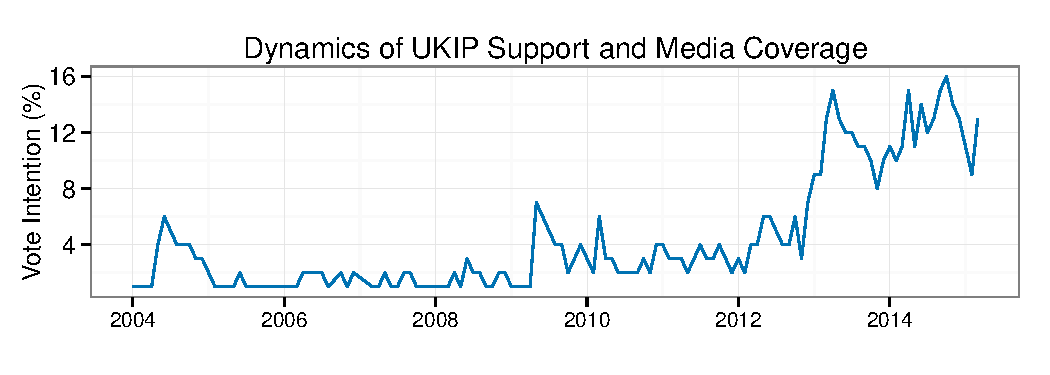
\includegraphics{ukip_media_files/figure-latex/unnamed-chunk-1-1.pdf}
\caption{}
\end{figure}

\begin{figure}[htbp]
\centering
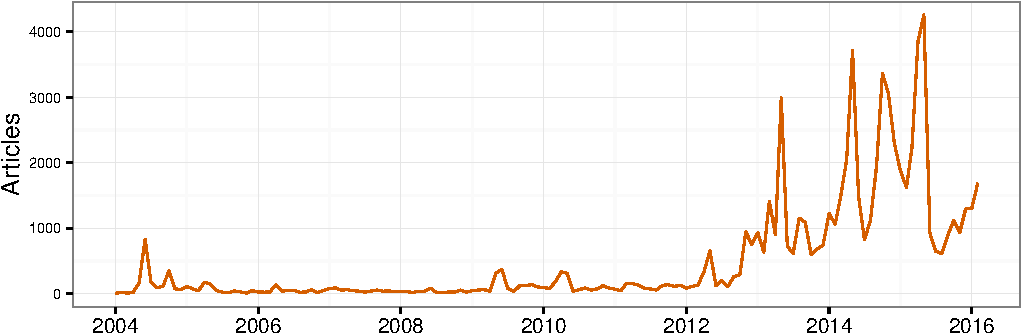
\includegraphics{ukip_media_files/figure-latex/unnamed-chunk-2-1.pdf}
\caption{}
\end{figure}

\begin{figure}[htbp]
\centering
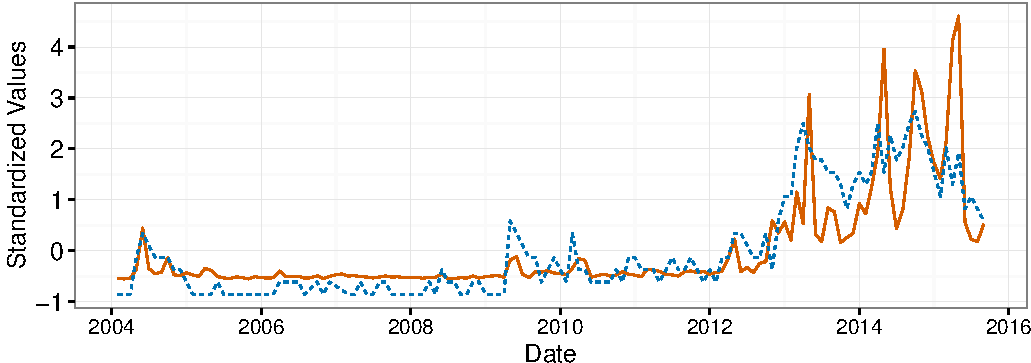
\includegraphics{ukip_media_files/figure-latex/unnamed-chunk-3-1.pdf}
\caption{Dynamics of UKIP Support and Media Coverage}
\end{figure}

\setlength\parindent{24pt}

The variable \emph{Articles} reflects the number of articles Nexis
returns from the first day of each month until the last day of each
month. Figure 1 provides a summary view of the two main variables of
interest. The dotted line represents \emph{Support} and the solid line
represents \emph{Articles}. Raw values are displayed in the first two
(top) panels. For ease of direct comparison the bottom panel displays
standardized scores in which each value is derived by subtracting the
mean of the particular time-series and dividing by one standard
devation.

It is also plausible that elections have an independent effect on
coverage and support due to general increased media attention and
campaigning. For this reason, we have included eponymous dummy variables
for the months of each national and European election within the
sampling period. The elections included are three European elections
(June 2004, June 2009 and May 2014) and three general elections (May
2005, May 2010, and May 2015). European elections coincide with local
elections in the UK.

In the present analysis we do not consider public opinion on particular
political issues, measures of objective political or policy dynamics, or
the visibility of party leaders in the media, for several reasons. The
first and main reason is dictated by our problem-driven approach.
Because our contribution to the literature is motivated by a particular
debate in the politics of British media, we focus on the parameters of
that debate, which have revolved around party coverage. Although UKIP's
controversial leader Nigel Farage is likely a significant aspect of
UKIP's media visibility, coverage of Farage is almost certainly highly
correlated with coverage of the party, as Vliegenhart, Boomgaarden, and
Van Spanje find of party and leader coverage in multiple other Western
European countries. Second, Vliegenhart, Boomgaarden, and Van Spanje
also find that media coverage of parties is, overall, more relevant than
party leader as a predictor of party support (Vliegenthart et al., 2012:
333). While it is possible that phenomena such as objective immigration
levels, media coverage of immigration, and/or public opinion on
immigration may affect both UKIP party coverage and public support for
UKIP, it is not theoretically straightforward that they should affect
one of our main variables more, or sooner, than the other. Because we
lack any particular theoretical perspective on such possibilities, and
there are many additional causal factors which could arguably be
included in this system, we refrain from proliferating additional
variables (Achen, 2006).

We first use econometric techniques to test for, and distinguish the
ordering of, potential causal dynamics between media coverage and public
support for UKIP. An ideal approach to testing the presented hypotheses
is vector autoregression (VAR) with Granger causality tests (Brandt and
Williams, 2007; Vliegenthart et al., 2012). Specifically, we estimate a
VAR by OLS per equation, using the following form:

\begin{equation}
 \label{eq:VAR}
    y_t = A_1 y_{t-1} + … + A_p y_{t-p} + D_t + u_t
\end{equation}

where \(y_t\) is a \(K \times 1\) vector of endogenous variables and
\(u_t\) is the error term. In our case the endogenous variables are
\emph{Support} and \emph{Articles}. The coefficient matrices \(A_1\),
…, \(A_p\) are of dimension \(K \times K\). By convention \(p\)
denotes the ``order'' of the VAR, or the number of lags used. Typically
this is determined empirically, as we do below. In addition, \(D_t\)
refers to a vector of exogenous regressors. In our case the exogenous
regressors include a constant term, a trend term, the dummy variable for
UK General Election months, and the dummy variable of European election
months. We then use the conventional F-type Granger-causality test for
each of the two endogenous variables in the system. The vector of
endogenous variables \(y_t\) is divided into two vectors \(y_1t\) and
\(y_2t\) of dimensionality (\(K_1 \times 1\)) and (\(K_2 \times 1\))
with \(K = K_1 + K_2\) (Pfaff, 2008). The null hypothesis is that no
lags of variable \(y_{1t}\) are significant in the equation for variable
\({y}_{2t}\). If \(\alpha_{21, i} = 0\) for \(i = 1\), \(2\), …,
\(p\), we say that \(y_{1t}\) does not ``Granger-cause'' \(y_{2t}\).

Additionally, a brief qualitative historical analysis of the dynamics is
conducted to further probe any potential causal process(es). It is
arguably a general blindspot of quantitative time-series research to
neglect inquiry into the subsantive historical processes corresponding
to the statistical properties of time-series data. In particular, the
substantive nature of the puzzle at hand requires the identification of
a historical narrative which would not necessarily follow from a
statistical fact such as Granger causality. Even with econometric
evidence suggesting an association in one direction or the other, it
would remain unclear whether the historical unfolding of such dynamics
may imply a substantively significant issue for the core democratic
function under consideration.

For instance, it could be the case that, formally, media coverage
Granger-causes public support \emph{and} that exogenous increases in
media coverage played no particularly important role in the rise of UKIP
support. This is because statistical properties of time-series in no way
preclude the fact that the historically key moments of UKIP's rise could
have been random or contingent consequences of other factors.
Additionally, it is always possible in any particular historical process
that \(Y_1\) has an average effect on \(Y_2\) which is statistically
significant but in key, contingent moments certain shifts in \(Y_2\) may
explain unique changes in \(Y_1\) in a fashion which is not
statistically distinguishable. In the latter case, media-caused
increases in public support might themselves be responding to, and
amplifying, contingent but exogenous increases in public support in an
arguably democracy-consistent fashion, even if increases in support do
not statistically predict increases in media coverage.

To provide the strongest possible investigation of the role media has
played in the rise of UKIP support, we will need to assess the degree to
which increases in media coverage were followed by increases in public
support for UKIP following \emph{stagnant or decreasing} levels of
support in preceding months. We will then also need to assess the degree
to which such identifiable historical moments were related to the
relatively few key moments in which support for UKIP rises most
dramatically. We explore these substantive questions with a brief but
detailed narrative of the political events and media themes which lie
behind our time-series data.

\section{Findings and Discussion}\label{findings-and-discussion}

Because both variables are non-stationary, vector autoregression is
estimated with first differences of each variable. Optimal lag length is
determined by the Aikeke Information Criterion to be VAR(3). The model
includes a constant and a trend term. Diagnostics suggest that using the
log of each variable before differencing reduces heteroskedasticity and
serial correlation of errors. The models displayed here all pass the
standard ARCH-LM and Portmanteau tests for non-constant error variance
and serial correlation of errors, respectively. Finally, diagnostics
show no evidence of significant temporal instability (see Supplementary
Information).

\begin{table}[!htbp] \centering 
  \caption{Vector Autoregression} 
  \label{} 
\begin{tabular}{@{\extracolsep{5pt}}lcc} 
\\[-1.8ex]\hline 
\hline \\[-1.8ex] 
 & \multicolumn{2}{c}{\textit{Dependent variable:}} \\ 
\cline{2-3} 
\\[-1.8ex] & \multicolumn{2}{c}{} \\ 
 & $\Delta Support$ & $\Delta Articles$ \\ 
\\[-1.8ex] & (1) & (2)\\ 
\hline \\[-1.8ex] 
 $\Delta Articles_{t-1}$ & 0.210$^{**}$ & $-$0.300$^{***}$ \\ 
  & (0.110) & (0.095) \\ 
  & & \\ 
 $\Delta Support_{t-1}$ & $-$0.460$^{***}$ & 0.019 \\ 
  & (0.096) & (0.086) \\ 
  & & \\ 
 $\Delta Articles_{t-2}$ & 0.180$^{**}$ & $-$0.260$^{***}$ \\ 
  & (0.093) & (0.083) \\ 
  & & \\ 
 $\Delta Support_{t-2}$ & $-$0.260$^{**}$ & $-$0.081 \\ 
  & (0.100) & (0.090) \\ 
  & & \\ 
 $\Delta Articles_{t-3}$ & 0.180$^{**}$ & $-$0.100 \\ 
  & (0.092) & (0.082) \\ 
  & & \\ 
 $\Delta Support_{t-3}$ & $-$0.080 & $-$0.063 \\ 
  & (0.094) & (0.084) \\ 
  & & \\ 
 Constant & 0.015 & 0.039 \\ 
  & (0.077) & (0.069) \\ 
  & & \\ 
 Trend & 0.00004 & $-$0.0001 \\ 
  & (0.001) & (0.001) \\ 
  & & \\ 
 General Elections & 0.120$^{*}$ & 0.330$^{***}$ \\ 
  & (0.059) & (0.053) \\ 
  & & \\ 
 EU Elections & 0.016 & 0.090 \\ 
  & (0.066) & (0.059) \\ 
  & & \\ 
\hline \\[-1.8ex] 
Observations & 141 & 141 \\ 
R$^{2}$ & 0.160 & 0.370 \\ 
Adjusted R$^{2}$ & 0.100 & 0.320 \\ 
Residual Std. Error (df = 131) & 0.440 & 0.390 \\ 
F Statistic (df = 9; 131) & 2.800$^{***}$ & 8.500$^{***}$ \\ 
\hline 
\hline \\[-1.8ex] 
\textit{Note:}  & \multicolumn{2}{r}{$^{*}$p$<$0.1; $^{**}$p$<$0.05; $^{***}$p$<$0.01} \\ 
\end{tabular} 
\end{table}

Initial VAR results show little evidence that changes in public support
predict media coverage, but statistically significant evidence that
media coverage drives public support. As the numerical results and the
Impulse Response plots show, there is no statistically discernable
correlation between past changes in public support and changes in media
coverage, whereas past changes in media coverage have a statistically
significant correlation with future changes in public support. As
reported in Table 2, Granger causality tests support this
interpretation, with the latter relationship identified in the model
very unlikely to be observed by chance alone (p\textless{}.05).

We note there are limitations of the data which may make it difficult to
identify the full range of causal effects in a VAR approach. First, it
is possible that monthly measures are too infrequent to capture causal
effects if the real lag between effects is shorter than one month. Also,
importantly, structural tests on all models suggest strong evidence of
instantaneous causality. Thus, the VAR results suggest clear but
imperfect and, for reasons discussed above, inherently limited evidence
for Hypothesis 1 that increases in media coverage lead to increases in
public support. The VAR results provide no evidence for Hypothesis 2,
that increases in public support lead to increases in media coverage.
Given the problem of instantaneous causality, we cannot rule out the
possibility that both variables drive each other in periods shorter than
one month or that both variables are driven by some third unobserved
variable. Nonetheless, the stylized empirical fact of our data is that
media coverage Granger-causes public support and not vice-versa.

\begin{table}[!htbp] \centering 
  \caption{Granger Causality Tests} 
  \label{} 
\begin{tabular}{@{\extracolsep{5pt}} ccc} 
\\[-1.8ex]\hline \\[-1.8ex] 
 & Support & Articles \\ 
\hline \\[-1.8ex] 
P-value & $0.034$ & $0.740$ \\ 
DF1 & $3$ & $3$ \\ 
DF2 & $262$ & $262$ \\ 
F-test & $2.900$ & $0.420$ \\ 
\hline \\[-1.8ex] 
\end{tabular} 
\end{table}

\begin{figure}[htbp]
\centering
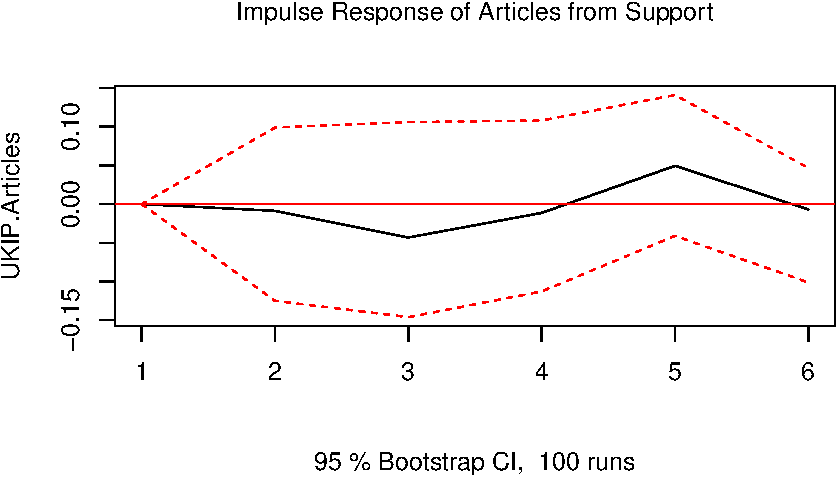
\includegraphics{ukip_media_files/figure-latex/unnamed-chunk-7-1.pdf}
\caption{Impulse Response Plot Shows Effect on Articles from an
Exogenous Increase in Support}
\end{figure}

\begin{figure}[htbp]
\centering
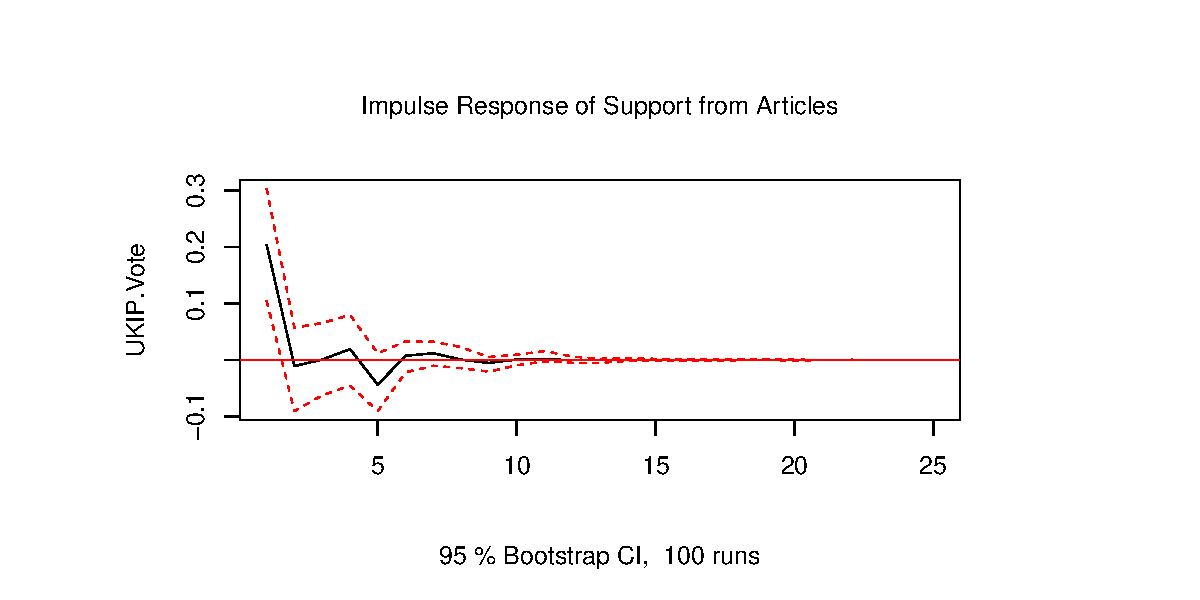
\includegraphics{ukip_media_files/figure-latex/unnamed-chunk-8-1.pdf}
\caption{Impulse Response Plot Shows Effect on Support from an Exogenous
Increase in Articles}
\end{figure}

\section{Qualitative Analysis}\label{qualitative-analysis}

To what extent are the statistical regularities identified by the vector
autoregression historically significant causal factors in the rise of
public support for UKIP? To facilitate a qualitative investigation of
the dynamics, we quantitatively identifed months which meet criteria
similar to the concept of Granger causality. Any month (\(t\)) that is
immediately preceded by two months (\(t-1\), \(t-2\)) of stagnating or
declining public support but increased media coverage, we designate as a
month of ``uncaused'' media increase or media ``bias'' for short.
Symmetrically, any month that is immediately preceded by two months of
stagnating or declining media coverage but increasing public support, we
consider a month of ``uncaused'' or exogenously increasing public
support. To mitigate the probability we will be counting mere noise as
meaningful increases, we count as increases only those greater than .05
standard deviations and all other months as ``stagnating or
decreasing.'' Figure 2 presents the standardized values of each time
series with dashed and green vertical lines indicating months of
uncaused media `bias' and grey, dotted vertical lines indicating months
of uncaused increases in public support. Even a first, superficial
consideration of Figure 2 reveals that increases in media coverage
unwarranted by public support are not only roughly as frequent as
uncaused increases in public support, but they are found at multiple
pivotal months in periods of the most dramatic increases in UKIP's
public support. To be clear, we are not claiming to pinpoint key moments
of causal effect; in any particular point of the time-series, it is
impossible to know whether a pattern is random noise or a true
``signal'' of one variable causing a change in another variable. Rather,
we take the evidence from the VAR to be our warrant for exploring the
qualitative data in search of possible examples whereby the substantive
significance of the statistical evidence may either be better
illustrated or possibly discounted due to untheorized contingencies.
Based on our preliminary explorations summarized in Figure 2, we focus
especially on two key periods: from July to September of 2012, and the
second half of 2013. We begin, however, with a brief history of the rise
of UKIP.

UKIP, formed in 1993, began fielding European parliamentary candidates
in 1994 and British parliamentary candidates in 1997. Since then, the
party has enjoyed mixed but notable increases in public support and in
electoral outcomes, particularly in the European parliament where the
party was the largest in the 2014 election. Until the 2015 general
election, UKIP’s domestic electoral success had been much less
impressive, receiving just 3.1\% of the vote in 2010. Like other small
or new parties, it has a history of infighting, changes of direction and
leadership, and problems with financial mismanagement (Whitaker and
Lynch, 2011). As recently as 2011, a lack of media attention was cited
as a factor in UKIP’s poor performance, as well as credibility and
relatively few activists (Ford et al., 2012). Indeed, the historical
pattern of both media coverage and public support for UKIP over much of
its recent history, from 2004 to 2009, was a series of small increases
which consistently returned to low baseline quantities of little
political consequences (Murphy, 2015).

The party experienced its first bump in both coverage and voting
intention in 2004 with the European election, in which they received
16\% of the vote, where coverage reached 829 articles in a single month,
their record amount of coverage at the time and the greatest amount of
coverage the party would experience until 2012. During this spike, both
media coverage and voting intention increase proportionately and as
would be expected if coverage was driven by public opinion: Figure 2
indicates no bias or exogenous increases of support in this instance.
Following this, both coverage and support decay and return to poltically
negligible levels. Over the next eight years, there are a range of
events that do not attract very much media attention or public support;
indeed, events occur between these years that are similar to those that
will occur in later years but they fail to generate the extraordinary
media attention gained by such events in later years. The vast majority
of coverage is ``in passing,'' such as everday reports of election
results, or else it is negative, regarding claims of fraud and
infighting. Indeed, Figure 2 shows that this period was characterised by
exogenous increases of support not tracked by media coverage, supporting
the claim that a lack of media coverage failed to facilitate public
support through this period (Ford et al., 2012). In some ways, the
identification of the two series following each other without any `bias'
and of exogenous increases of support gives us some confidence in the
findings of bias discussed earlier.

Apart from the 2005 election, in which UKIP received little coverage and
performed poorly (receiving just 149 articles in that month) (Anon.,
2005; Morris, 2005), UKIP saw little change in public support or media
coverage until the European elections of 2009. There is a small boost in
both support and coverage in April 2006, when David Cameron calls the
party ‘fruitcakes, loonies’ and ‘closet racists’ (White and
Watt, 2006). Interestingly, this rise in media coverage was followed by
a small but sustained boost in public support, which persisted for three
months. In April 2008, Conservative MP Bob Spink defected, giving UKIP
their first MP which generated very little coverage, despite being
called a coup (Winnett and Prince, 2008). Even the European election in
2009, in which UKIP came in second place, generated far less coverage
than the 2005 European election, where the party came in third place
(829 to 320 articles in a month, respectively). Despite this, it was
still hailed as a ‘political earthquake’ (Watt and Taylor, 2009) and
garnered coverage for UKIP’s leader Nigel Farage.

\begin{figure}[htbp]
\centering
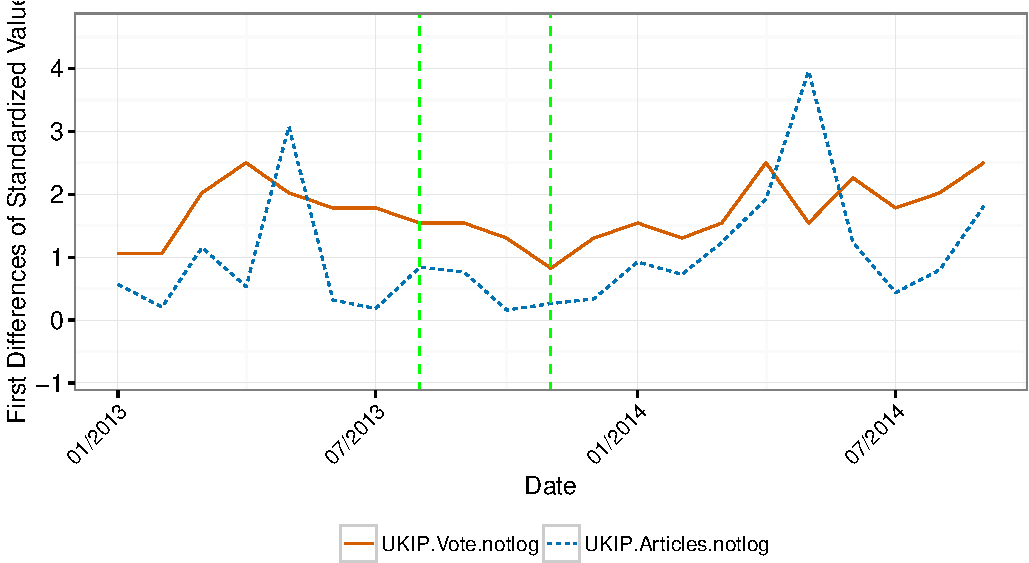
\includegraphics{ukip_media_files/figure-latex/unnamed-chunk-9-1.pdf}
\caption{Standardized Time-Series, Green Lines Indicate Media ``Bias''
and Grey Lines Indicate Exogenous Increases in Support}
\end{figure}

\begin{figure}[htbp]
\centering
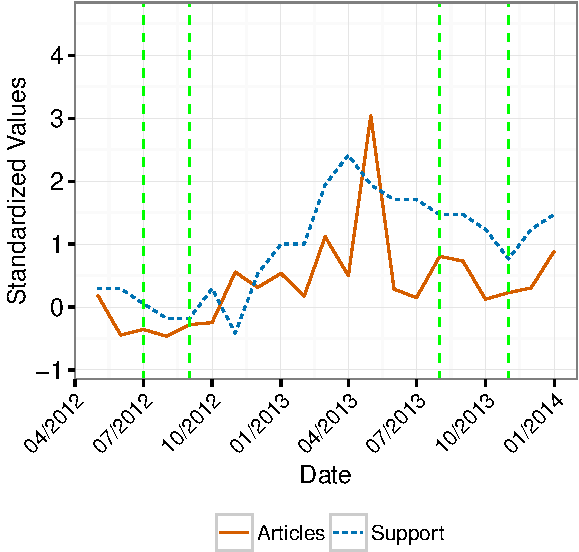
\includegraphics{ukip_media_files/figure-latex/unnamed-chunk-10-1.pdf}
\caption{Standardized Time-Series, April 2012 to January 2014}
\end{figure}

Following this, there are at least two occasions where media coverage
both precedes and seems unrelated to UKIP's public support, which may
then have generated further increases in popular support (Murphy, 2015).
To aid our investigation, we refer to Figure 5, which shows Figure 4 at
higher resolution for the months between May 2012 and January 2014. This
period includes a three by-elections (Corby, Middlesborough and
Rotherham), with many being controversial (Wainwright, 2012), as well as
the UKIP party conference. All three of these by-elections occurred in
November 2012, and UKIP placed second in two and third in Corby, with
the Rotherham by- election's 21\% vote share being the party's highest
up to that point. In July 2012 UKIP's public support was unremarkably
near its average and was declining from June, after it had been stagnant
since May. But media coverage held relatively steady, slightly
decreasing once but slightly increasing twice (and slightly increasing
overall) from June to September, from 123 to 261 articles. It is only at
this point that public support increases notably from September to
October and is followed by a spike in media coverage that likely
represented a moment of positive feedback ending in the first truly
significant rise of UKIP into mainstream public consciousness - up to
15\% support in April 2013.

Between August and November 2012, the amount of articles covering UKIP
increased from 198 to 948, the most they had ever received in one month
at the time, beyond three standard deviations from their long-term mean.
To be clear, this dramatic surge of UKIP support appears to launch with
a moment of postive feedback betwen support and media coverage,
genuinely containing a notable spike of public support at the beginning.
However, the main quantitative and qualitative implication of this
particular period, is that the months of July and September 2012 are
months in which media coverage is slightly increasing despite stagnant
or declining levels of public support, and it is these dynamically
unresponsive months of media coverage that precede the spike in support
observed in October. Of course, it is impossible to distinguish these
slight increases in media coverage in July and September from random
noise in the polling; but from the statistical analysis we have reason
to believe such moments of unresponsively increasing media coverage are
at least comparatively more likely to be predictve of changes in support
than vice versa. Thus, while it would be impossible to demonstrate
conclusively that these months of media coverage played a causal role in
the dramatic rise of support achieved by November, our model suggests it
is more likely these unresponsively stable and slightly increasing
months of media coverage played a causal role in the increased support
of October, than it is that the increased support in October played a
causal role in the then-highest level of media coverage seen in
November. In turn, the unprecedently high levels of media coverage in
November likely played more of a role in the following spike of support
than the October spike in support played in the November spike in media
coverage. This interpretation is enhanced by the additional fact that
after the spike in support of October, November returned to the lowest
level of support observed in several months. Again, while we cannot
confidently read causal dynamics in particular data points, the point is
that the increase in support of October, which ostensibly seems to be
followed by a spike in media coverage ultimately leading to UKIP's real
debut, is a less plausible interpretation of the data than one based on
Hypothesis 1.

Now consider the period between July 2013 and December 2014. Despite
public support declining rapidly and steadily from its high point in
April 2013, media coverage from July to August increases considerably,
from 613 to 1154 articles in the month. Public support continues to
decline through August until November, decreasing from 11\% to 8\%.
While media coverage appears to adjust dynamically downward after it's
``uncaused'' increase of August, yet again in November media coverage
stabilizes and slightly increases. It is only at this point in November
that support ends its long and steady decline and yet again begins
another substantial increase until it returns back to the high levels of
April 2013. Again, in these two months we identify apparently minor but
potentially crucial non-dynamically-responsive levels of media coverage
which may be functioning as a floor preventing support from continuing
to decline and making possible the surge beginning from November 2013.
While of course these spikes and drops in support may just be volatility
around UKIP's new, higher mean levels of support, the key point here is
only to explore and give possible instances of the statistical findings.
Unlike the previous instance of ``bias'' explored above, where political
events such as by-elections and the party conference season may have
played roles, in this case there are no obvious and directly
party-related events shaping the dynamics in this period. However, one
key event which may have played a role at this time is the lifting of
work restrictions on Romanian and Bulgarian nationals which occurred in
January 2014 (Martin, 2013), with media coverage intensifying in the
months leading up to January. The increased salience of issues related
to migration and the European Union may help to explain changes in media
coverage independent of UKIP's support. Interestingly, considerable
coverage also surrounded Farage's comment, in December 2013, that
Britain should accept Syrian refugees (Goodman, 2013).

Previous studies have relied on statistical models similar to the one we
have presented here. However, this may ignore interesting dynamics
hidden within the data about what is happening in the relationship
between media coverage and public opinion. A qualitative appreciation of
the data indicates at least two key examples where increased media
coverage unwarranted by changes in public support take place in key
periods of UKIP's rise.

\section{Conclusion}\label{conclusion}

This study has made three contributions. Firstly, to our knowledge this
is one of the first articles to study the dynamics of right-wing
populist party support and quantity of media coverage in the context of
a majoritarian system and the UK in particular; previous research has
primarily focused on other Western European democracies such as Belgium,
the Netherlands and Germany. Despite the change in political system, our
findings support those of (Vliegenthart and Boomgaarden, 2010;
Vliegenthart et al., 2012), as we find quantitative and qualitative
evidence that media coverage has played a unique causal role in
increasing support for UKIP, in a fashion irreducible to previous levels
of support or election outcomes.

Secondly, this article contributes to currently on-going efforts to
advance the methodological aspects of research on media and public
opinion (Vliegenthart, 2014). Unlike many quantitative studies, we
provide an analytically sophisticated qualitative investigation of our
statistical findings. Most previous research on the visibility-support
nexus relies primarily on statistical evidence, which cannot necessarily
address important questions relating to the substantive historical
narrative of a particular political party. We find that, in two periods,
increases in media coverage came after two months of stagnating or
declining public support but was then followed by historically pivotal
increases in support. While we cannot claim these periods are definitive
instances of causality, they show that the particular and contingent
historical unfolding of UKIP is consistent with the inference, suggested
by our statistical analysis, that media coverage played a unique and
important causal role in the rise of public support for UKIP.

Perhaps most importantly, these findings are of significance to
contemporary public debate in the UK concerning the perception that
unfair quantities of media coverage are given to UKIP. Some have argued
that extensive media coverage of UKIP is justified due to public support
for the party. The findings here, on the other hand, suggest this is an
unacceptable argument: the extraordinary media coverage which has been
given to UKIP cannot be explained or defended on grounds of public
support. We find that media coverage has no reliable relationship to
public support in the one month, two months, or three months before a
particular month of coverage. Indeed, we find that coverage may have
independently and uniquely driven some of the very public support which
media regulators would later point to as their justification for the
extraordinary coverage given to UKIP. Our findings therefore raise
serious questions for the function of media coverage in a democratic
political system, because they suggest that unelected and
unrepresentative actors (the media) may be systematically shaping public
opinion toward, and the fortunes of, certain political parties in
contradiction to organic levels of public support for those parties.

As with all studies, there are limitations to the present study and
certain areas for future research may be indicated. We have left aside
the question of leader effects, given previously ambiguous findings. We
do not undertake any form of content analysis to address the actual
content of the coverage in question, but only look at the quantity of
articles. It is possible that, by disaggregating the coverage further,
different types of coverage may have different effects; it would also be
interesting to see whether the positivity or negativity of coverage
matters for future levels of public support. Similarly, we do not
disaggregate between types of newspapers, such as broadsheet or tabloid,
which may offer different types of coverage and have different effects.
We also only focus on print media. This means that we have not accounted
for the effect of visual and social media which may play a role in
dynamics of party support.

\pagebreak

\section{Supplementary Information}\label{supplementary-information}

\begin{figure}[htbp]
\centering
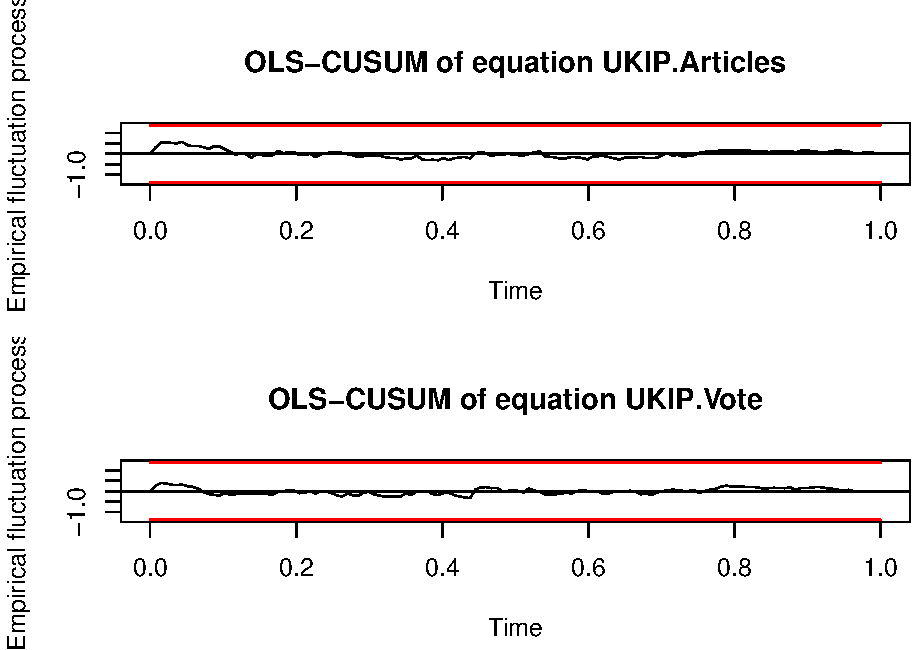
\includegraphics{ukip_media_files/figure-latex/supplementary-1.pdf}
\caption{}
\end{figure}

\pagebreak

\section{References}\label{references}

\singlespacing

\raggedright

\setlength\parindent{0pt}

\hyperdef{}{ref-Achen:2006fp}{\label{ref-Achen:2006fp}}
Achen, Christopher H. (2006) ``Let's Put Garbage-Can Regressions and
Garbage-Can Probits Where They Belong.'' \emph{Conflict Management and
Peace Science} 22:327--339.

\hyperdef{}{ref-althausux5fusingux5f2001}{\label{ref-althausux5fusingux5f2001}}
Althaus, Scott L., Jill A. Edy, and Patricia F. Phalen. (2001) ``Using
Substitutes for Full-Text News Stories in Content Analysis: Which Text
Is Best?'' \emph{American Journal of Political Science} 45:707--723.
\url{http://www.jstor.org/stable/2669247} (Accessed February 23, 2016).

\hyperdef{}{ref-ux5felectionux5f2005}{\label{ref-ux5felectionux5f2005}}
Anon. (2005) ``Election 2005: UKIP and Greens fail to make gains.''
\emph{The Guardian}.

\hyperdef{}{ref-Baum:2012je}{\label{ref-Baum:2012je}}
Baum, Matthew A. (2012) ``The Iraq Coalition of the Willing and
(Politically) Able: Party Systems, the Press, and Public Influence on
Foreign Policy.'' \emph{American Journal of Political Science}
57:442--458.

\hyperdef{}{ref-BBC:R6UMvIKM}{\label{ref-BBC:R6UMvIKM}}
BBC. (2015) ``Appendix I Party Coverage 2015.''
\url{http://downloads.bbc.co.uk/bbctrust/assets/files/pdf/our_work/election_guidelines/2015/draft_election_guidelines_appendix.pdf}.

\hyperdef{}{ref-beckux5fsocialux5f2002}{\label{ref-beckux5fsocialux5f2002}}
Beck, Paul Allen, Russell J. Dalton, Steven Greene, and Robert
Huckfeldt. (2002) ``The Social Calculus of Voting: Interpersonal, Media,
and Organizational Influences on Presidential Choices.'' \emph{The
American Political Science Review} 96:57--73.
\url{http://www.jstor.org/stable/3117810} (Accessed October 26, 2015).

\hyperdef{}{ref-Benson:2009kb}{\label{ref-Benson:2009kb}}
Benson, Rodney. (2009) ``What makes news more multiperspectival? A field
analysis.'' \emph{Poetics} 37:402--418.
\url{http://linkinghub.elsevier.com/retrieve/pii/S0304422X09000412}.

\hyperdef{}{ref-Boomgaarden:2007ia}{\label{ref-Boomgaarden:2007ia}}
Boomgaarden, Hajo G, and Rens Vliegenthart. (2007) ``Explaining the rise
of anti-immigrant parties: The role of news media content.''
\emph{Electoral Studies} 26:404--417.

\hyperdef{}{ref-Boomgaarden:2009ke}{\label{ref-Boomgaarden:2009ke}}
Boomgaarden, Hajo G, and Rens Vliegenthart. (2009) ``How news content
influences anti-immigration attitudes: Germany, 19932005.''
\emph{European Journal of Political Research} 48:516--542.

\hyperdef{}{ref-Bos:2011iy}{\label{ref-Bos:2011iy}}
Bos, Linda, Wouter van der Brug, and Claes de Vreese. (2011) ``How the
Media Shape Perceptions of Right-Wing Populist Leaders.''
\emph{Political Communication} 28:182--206.

\hyperdef{}{ref-brandt2007multiple}{\label{ref-brandt2007multiple}}
Brandt, Patrick T, and John Taylor Williams. 2007. \emph{Multiple time
series models}. London: Sage.

\hyperdef{}{ref-daltonux5fpartisanux5f1998}{\label{ref-daltonux5fpartisanux5f1998}}
Dalton, Russell J., Paul A. Beck, and Robert Huckfeldt. (1998)
``Partisan Cues and the Media: Information Flows in the 1992
Presidential Election.'' \emph{The American Political Science Review}
92:111--126. \url{http://www.jstor.org/stable/2585932} (Accessed October
3, 2015).

\hyperdef{}{ref-deaconux5fukux5f2015}{\label{ref-deaconux5fukux5f2015}}
Deacon, David, and Dominic Wring. (2015) ``The UK Independence Party,
populism and the British news media: Competition, collaboration or
containment?'' \emph{European Journal of Communication}
0267323115612215.
\url{http://ejc.sagepub.com/content/early/2015/11/06/0267323115612215}
(Accessed February 23, 2016).

\hyperdef{}{ref-Duverger:1972wk}{\label{ref-Duverger:1972wk}}
Duverger, Maurice. (1972) ``Factors in a two-party and multiparty
system.'' \emph{Party politics and pressure groups}. New York
\url{http://scholar.google.com/scholar?q=related:rSp_PasTzcEJ:scholar.google.com/\&hl=en\&num=20\&as_sdt=0,5}.

\hyperdef{}{ref-fordux5fstrategicux5f2012}{\label{ref-fordux5fstrategicux5f2012}}
Ford, Robert, Matthew J. Goodwin, and David Cutts. (2012) ``Strategic
Eurosceptics and polite xenophobes: Support for the United Kingdom
Independence Party (UKIP) in the 2009 European Parliament elections.''
\emph{European Journal of Political Research} 51:204--234.
\url{http://onlinelibrary.wiley.com/doi/10.1111/j.1475-6765.2011.01994.x/abstract}
(Accessed November 16, 2015).

\hyperdef{}{ref-Gerring:2015ub}{\label{ref-Gerring:2015ub}}
Gerring, John. (2015) ``The relevance of relevance.'' In: Gerry Stoker,
Guy B Peters, and Jon Pierre (eds) \emph{The relevance of political
science}. London: Palgrave Macmillan
\url{http://blogs.bu.edu/jgerring/files/2014/11/Chapter-2.pdf}.

\hyperdef{}{ref-goodmanux5fdoesux5f2013}{\label{ref-goodmanux5fdoesux5f2013}}
Goodman, Paul. (2013) ``Does Mr Farage want to destroy the
Conservatives, or join them?; By urging ministers to accept Syrian
refugees, Ukip's leader has played a very canny game.'' \emph{The Daily
Telegraph}.

\hyperdef{}{ref-Goodwin:03LtHfhh}{\label{ref-Goodwin:03LtHfhh}}
Goodwin, Matthew, and Robert Ford. (2013) ``Just how much media coverage
does UKIP get?'' \emph{New Statesman}.
\url{http://www.newstatesman.com/politics/2013/11/just-how-much-media-coverage-does-ukip-get}.

\hyperdef{}{ref-hopmannux5feffectsux5f2010}{\label{ref-hopmannux5feffectsux5f2010}}
Hopmann, David Nicolas, Rens Vliegenthart, Claes De Vreese, and Erik
Albæk. (2010) ``Effects of Election News Coverage: How Visibility and
Tone Influence Party Choice.'' \emph{Political Communication}
27:389--405. \url{http://dx.doi.org/10.1080/10584609.2010.516798}
(Accessed October 10, 2015).

\hyperdef{}{ref-IpsosMORI:gm2fXYNK}{\label{ref-IpsosMORI:gm2fXYNK}}
Ipsos-MORI. (n.d.) ``Voting Intention in Great Britain: Recent Trends.''
\url{https://www.ipsos-mori.com/researchpublications/researcharchive/poll.aspx?oItemId=107\&view=wide}.

\hyperdef{}{ref-koopmansux5friseux5f2009}{\label{ref-koopmansux5friseux5f2009}}
Koopmans, Ruud, and Jasper Muis. (2009) ``The rise of right-wing
populist Pim Fortuyn in the Netherlands: A discursive opportunity
approach.'' \emph{European Journal of Political Research} 48:642--664.
\url{http://onlinelibrary.wiley.com/doi/10.1111/j.1475-6765.2009.00846.x/abstract}
(Accessed October 10, 2015).

\hyperdef{}{ref-Kumlin:2001iq}{\label{ref-Kumlin:2001iq}}
Kumlin, Staffan. (2001) ``IdeologyDriven opinion formation in Europe:
The case of attitudes towards the third sector in Sweden.''
\emph{European Journal of Political Research} 39:487--518.
\url{http://onlinelibrary.wiley.com.libproxy.temple.edu/doi/10.1111/1475-6765.00585/abstract}.

\hyperdef{}{ref-martinux5fimmigrationux5f2013}{\label{ref-martinux5fimmigrationux5f2013}}
Martin, Iain. (2013) ``Immigration from Romania and Bulgaria set to give
Nigel Farage and Ukip a boost.'' \emph{The Telegraph}.
\url{http://blogs.telegraph.co.uk/news/iainmartin1/100252078/immigration-from-romania-and-bulgaria-set-to-give-nigel-farage-and-ukip-a-boost/}.

\hyperdef{}{ref-morrisux5felectionux5f2005}{\label{ref-morrisux5felectionux5f2005}}
Morris, Nigel. (2005) ``Election 2005: UKIP's bubble may have burst, but
Kilroy-Silk's party also fails to take off.'' \emph{The Independent}.

\hyperdef{}{ref-murphyux5fukipux5f2015}{\label{ref-murphyux5fukipux5f2015}}
Murphy, Justin. (2015) ``Ukip don't deserve their media prominence.
Here's the proof.'' \emph{New Statesman}.
\url{http://www.newstatesman.com/politics/2015/04/ukip-dont-deserve-their-media-prominence-heres-proof}.

\hyperdef{}{ref-norrisux5fvirtuousux5f2000}{\label{ref-norrisux5fvirtuousux5f2000}}
Norris, Pippa. 2000. \emph{A Virtuous Circle: Political Communications
in Postindustrial Societies}. Cambridge, UK: Cambridge University Press
\url{http://www.cambridge.org/gb/academic/subjects/politics-international-relations/comparative-politics/virtuous-circle-political-communications-postindustrial-societies}.

\hyperdef{}{ref-oegemaux5fpersonalizationux5f2009}{\label{ref-oegemaux5fpersonalizationux5f2009}}
Oegema, Dirk, and Jan Kleinnijenhuis. (2009) ``Personalization in
political Television News: A 13-Wave Survey Study to Assess Effects of
Text and Footage.'' \emph{Communications} 25:43--60.
\url{http://www.degruyter.com/view/j/comm.2000.25.issue-1/comm.2000.25.1.43/comm.2000.25.1.43.xml}
(Accessed October 26, 2015).

\hyperdef{}{ref-Ofcom:2015tt}{\label{ref-Ofcom:2015tt}}
Ofcom. (2015) ``Ofcom list of major parties.''
\url{http://stakeholders.ofcom.org.uk/binaries/broadcast/guidance/major-parties.pdf}.

\hyperdef{}{ref-paletzux5fpoliticalux5f1996}{\label{ref-paletzux5fpoliticalux5f1996}}
Paletz, David. 1996. \emph{Political communication research: Vol. 2.
Approaches, studies, assessments}. Norwood, NJ: Ablex.

\hyperdef{}{ref-pauwelsux5freassessingux5f2010}{\label{ref-pauwelsux5freassessingux5f2010}}
Pauwels, Teun. (2010) ``Reassessing conceptualization, data and
causality: A critique of Boomgaarden and Vliegenthart's study on the
relationship between media and the rise of anti-immigrant parties.''
\emph{Electoral Studies} 29:269--275.
\url{http://www.sciencedirect.com/science/article/pii/S0261379410000120}
(Accessed October 10, 2015).

\hyperdef{}{ref-Pfaff:2008wk}{\label{ref-Pfaff:2008wk}}
Pfaff, Bernhard. (2008) ``VAR, SVAR and SVEC Models: Implementation
Within R Package \emph{vars}.'' \emph{Journal of Statistical Software}
27.

\hyperdef{}{ref-rooduijnux5fmesmerisingux5f2014}{\label{ref-rooduijnux5fmesmerisingux5f2014}}
Rooduijn, Matthijs. (2014) ``The Mesmerising Message: The Diffusion of
Populism in Public Debates in Western European Media.'' \emph{Political
Studies} 62:726--744.
\url{http://onlinelibrary.wiley.com/doi/10.1111/1467-9248.12074/abstract}
(Accessed October 2, 2015).

\hyperdef{}{ref-sellersux5fwinningux5f2007}{\label{ref-sellersux5fwinningux5f2007}}
Sellers, Patrick J., and Brian F. Schaffner. (2007) ``Winning Coverage
in the U.S. Senate.'' \emph{Political Communication} 24:377--391.
\url{http://dx.doi.org/10.1080/10584600701641516} (Accessed October 11,
2015).

\hyperdef{}{ref-semetkoux5fgermanysux5f1994}{\label{ref-semetkoux5fgermanysux5f1994}}
Semetko, Holli A, and Klaus Schoenbach. 1994. \emph{Germany's Unity
Election: Voters and the Media}. Cresskill: Hampton Press.

\hyperdef{}{ref-Sheafer:2009hi}{\label{ref-Sheafer:2009hi}}
Sheafer, Tamir, and Gadi Wolfsfeld. (2009) ``Party Systems and
Oppositional Voices in the News Media A Study of the Contest over
Political Waves in the United States and Israel.'' \emph{The
International Journal of Press/Politics} 14:146--165.
\url{http://hij.sagepub.com/cgi/doi/10.1177/1940161209333089}.

\hyperdef{}{ref-Soussi:vy}{\label{ref-Soussi:vy}}
Soussi, Alasdair. (2014) ``Did British media help the UKIP win EU
poll?''
\url{http://www.aljazeera.com/indepth/features/2014/06/did-british-media-help-ukip-win-eu-poll-20146313346918679.html}.

\hyperdef{}{ref-Stevenson:wo}{\label{ref-Stevenson:wo}}
Stevenson, Alex. (2014) ``Caroline Lucas points finger at media's Farage
obsession.''
\url{http://www.politics.co.uk/news/2014/05/29/ukip-victory-caroline-lucas-points-finger-at-media-s-farage}.

\hyperdef{}{ref-Stromback:2006ht}{\label{ref-Stromback:2006ht}}
Strömbäck, Jesper, and Daniela V Dimitrova. (2006) ``Political and Media
Systems Matter A Comparison of Election News Coverage in Sweden and the
United States.'' \emph{The International Journal of Press/Politics}
11:131--147.
\url{http://hij.sagepub.com.libproxy.temple.edu/content/11/4/131.abstract}.

\hyperdef{}{ref-Sweeney:wp}{\label{ref-Sweeney:wp}}
Sweeney, Mark. (2015) ``BBC prepares to boost Ukip coverage as it ranks
it a larger party in election.''
\url{http://www.theguardian.com/media/2015/jan/15/bbc-prepares-to-boost-ukip-coverage-as-it-ranks-it-a-larger-party-in-election}.

\hyperdef{}{ref-treschux5fpoliticiansux5f2009}{\label{ref-treschux5fpoliticiansux5f2009}}
Tresch, Anke. (2009) ``Politicians in the Media: Determinants of
Legislators' Presence and Prominence in Swiss Newspapers.'' \emph{The
International Journal of Press/Politics} 14:67--90.
\url{http://hij.sagepub.com/content/14/1/67} (Accessed October 11,
2015).

\hyperdef{}{ref-Vliegenthart:2014di}{\label{ref-Vliegenthart:2014di}}
Vliegenthart, Rens. (2014) ``Moving up. Applying aggregate level time
series analysis in the study of media coverage.'' \emph{Quality \&
Quantity} 48:2427--2445.

\hyperdef{}{ref-vliegenthartux5fwhyux5f2010}{\label{ref-vliegenthartux5fwhyux5f2010}}
Vliegenthart, Rens, and Hajo G. Boomgaarden. (2010) ``Why the media
matter after all: A response to Pauwels.'' \emph{Electoral Studies}
29:719--723.
\url{http://www.sciencedirect.com/science/article/pii/S0261379410000855}
(Accessed October 11, 2015).

\hyperdef{}{ref-vliegenthartux5fanti-immigrantux5f2012}{\label{ref-vliegenthartux5fanti-immigrantux5f2012}}
Vliegenthart, Rens, Hajo G. Boomgaarden, and Joost Van Spanje. (2012)
``Anti-Immigrant Party Support and Media Visibility: A Cross-Party,
Over-Time Perspective.'' \emph{Journal of Elections, Public Opinion and
Parties} 22:315--358.
\url{http://dx.doi.org/10.1080/17457289.2012.693933} (Accessed October
10, 2015).

\hyperdef{}{ref-wainwrightux5frotherhamux5f2012}{\label{ref-wainwrightux5frotherhamux5f2012}}
Wainwright, Martin. (2012) ``Rotherham byelection brings relief for
Labour as Ukip celebrates second place.'' \emph{The Guardian}.
\url{http://www.theguardian.com/politics/2012/nov/30/rotherham-byelection-labour-ukip}.

\hyperdef{}{ref-walgraveux5fmakingux5f2004}{\label{ref-walgraveux5fmakingux5f2004}}
Walgrave, Stefaan, and Knut De Swert. (2004) ``The Making of the (Issues
of the) Vlaams Blok.'' \emph{Political Communication} 21:479--500.
\url{http://dx.doi.org/10.1080/10584600490522743} (Accessed October 10,
2015).

\hyperdef{}{ref-wattux5feuropeanux5f2009}{\label{ref-wattux5feuropeanux5f2009}}
Watt, Nicholas, and Matthew Taylor. (2009) ``European Elections: Ukip:
Eurosceptics claim second place is political earthquake.'' \emph{The
Guardian}.

\hyperdef{}{ref-Whitaker:2011gi}{\label{ref-Whitaker:2011gi}}
Whitaker, Richard, and Philip Lynch. (2011) ``Explaining Support for the
UK Independence Party at the 2009 European Parliament Elections.''
\emph{Journal of Elections, Public Opinion \& Parties} 21:359--379.
\url{http://www.tandfonline.com/doi/abs/10.1080/17457289.2011.588439}.

\hyperdef{}{ref-whiteux5fukipux5f2006}{\label{ref-whiteux5fukipux5f2006}}
White, Michael, and Nicholas Watt. (2006) ``Ukip threatens to sue over
Cameron's 'racist' remark.'' \emph{The Guardian}.
\url{http://www.theguardian.com/uk/2006/apr/05/otherparties.politics}
(Accessed November 16, 2015).

\hyperdef{}{ref-winnettux5ftoryux5f2008}{\label{ref-winnettux5ftoryux5f2008}}
Winnett, Robert, and Rosa Prince. (2008) ``Tory defector becomes Ukip's
first MP.'' \emph{The Daily Telegraph}.

\hyperdef{}{ref-Wintour:vf}{\label{ref-Wintour:vf}}
Wintour, Patrick. (2015) ``Ofcom deals blow to Greens election debate
hopes but boosts Ukips.''
\url{http://www.theguardian.com/politics/2015/jan/08/ofcom-blow-green-party-election-debate-boost-ukips}.

\end{document}
